% Página
\section{Fundamentos de Proteção}
\subsection{O que é Confidencialidade e por que importa}

A Confidencialidade refere-se à garantia de que as informações são acessíveis apenas por pessoas autorizadas. Em outras palavras, é a proteção contra a divulgação não autorizada de dados. Este pilar é essencial para manter a privacidade dos dados pessoais e sensíveis, como informações financeiras, médicas ou estratégicas de uma organização. Técnicas de criptografia são amplamente utilizadas para garantir a confidencialidade, assegurando que, mesmo que os dados sejam interceptados, eles não possam ser lidos ou compreendidos por indivíduos não autorizados.

\subsection{Como funcionam os Algoritmos Simétricos}

Entre os diversos tipos de algoritmos de criptografia, o algoritmo de criptografia simétrica é um dos mais comuns e amplamente utilizados. Neste tipo de algoritmo, a mesma chave(K) é utilizada tanto para criptografar(C), gerando a mensagem cifrada(M), quanto para descriptografar(D) os dados, gerando o Texto Plano(T).\\

A Figura \ref{fig:algoritmo_simetrico} ilustra o funcionamento do algoritmo de criptografia simétrica. Para mostrar o funcionamento do algoritmo, vamos considerar três personagens: \textbf{Alice}, \textbf{Bob} e \textbf{Eva}. Alice e Bob desejam se comunicar de forma segura, enquanto Eva deseja ler a mensagem trocadas entre eles.

\begin{figure}[H]
	\centering
	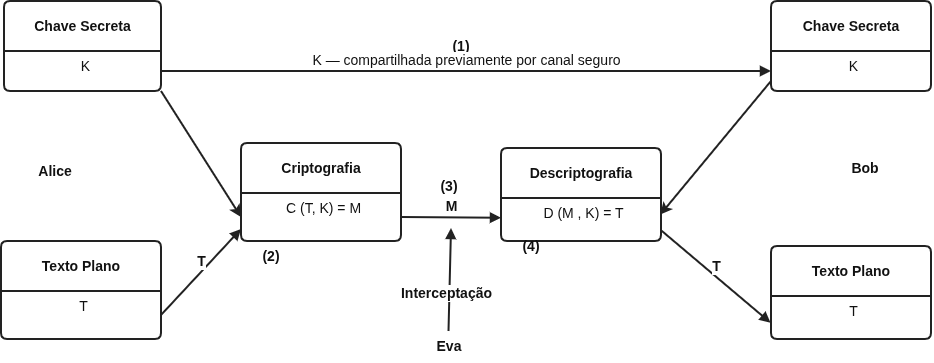
\includegraphics[scale=0.45]{algoritmo_simetrico.png}
	\caption{Funcionamento do algoritmo de criptografia simétrico}
	\label{fig:algoritmo_simetrico}
\end{figure}

A principal vantagem dos algoritmos de criptografia simétrica é sua eficiência e velocidade, especialmente em comparação com os algoritmos de criptografia assimétrica. No entanto, um dos desafios mais significativos é a distribuição segura da chave secreta. Se Eva conseguir interceptar ou descobrir a chave secreta, toda a comunicação entre Alice e Bob será comprometida.\\

Pelo motivo descrito acima, é essencial que Alice e Bob utilizem métodos seguros para compartilhar a chave secreta e garantam que ela permaneça protegida contra acessos não autorizados.

\subsection{A evolução: Key-Encryption-Key}

O conceito de Key-Encryption-Key, ou Chave de Criptografia de Chaves, é uma tecnologia utilizada para proteger outras chaves criptográficas, como por exemplo, o uso da KEK para proteger as Chaves de Criptografia de Dados(DEK). Ao usar uma KEK para resguardar as DEKs, adiciona-se uma camada extra de segurança ao sistema, melhorando significativamente sua proteção como um todo.\\

A Figura \ref{fig:kek} ilustra o funcionamento e da utilização do conceito KEK.

\begin{figure}[H]
	\centering
	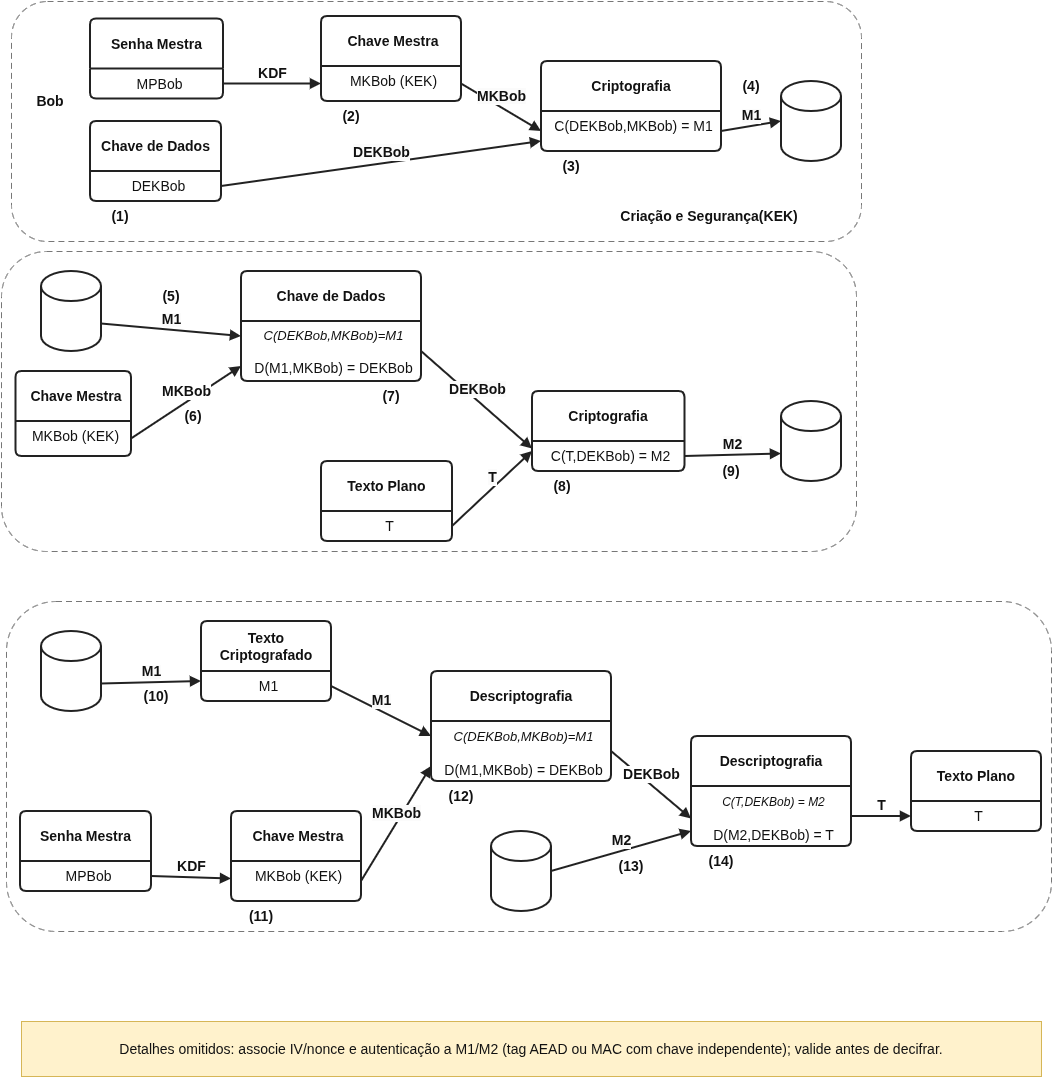
\includegraphics[scale=0.45]{kek.png}
	\caption{Funcionamento do conceito Key-Encryption-Key}
	\label{fig:kek}
\end{figure}

O Key-Encryption-Key é um componente essencial em arquiteturas de segurança que exigem a proteção de múltiplas chaves criptográficas \textbf{DEK}. Seu uso permite a proteção eficiente das DEKs, garantindo a segurança dos dados criptografados e simplificando a gestão das chaves. Implementar KEKs corretamente é necessário para manter a integridade e a confidencialidade dos dados em qualquer sistema seguro.\\

\pagebreak
